% \section{Metodología}
\section{Methodology}

% La metodología adoptada sigue el ciclo de vida estándar de un proyecto de aprendizaje automático, estructurándose en cuatro fases principales: preparación de datos, modelado y experimentación, estrategia de entrenamiento y despliegue. El enfoque se centró en superar las limitaciones de los detectores tradicionales en escenarios de alta densidad mediante la implementación de arquitecturas basadas en Transformers con optimización de arquitectura neuronal (NAS).
The adopted methodology follows the standard life cycle of a machine learning project, structured in four main phases: data preparation, modeling and experimentation, training strategy, and deployment. The approach focused on overcoming the limitations of traditional detectors in high-density scenarios through the implementation of Transformer-based architectures with Neural Architecture Search (NAS).

% \subsection{Gestión y Procesamiento de Datos}
\subsection{Data Management and Processing}

% \subsubsection{Descripción del Dataset}
\subsubsection{Dataset Description}

% Se utilizó el conjunto de datos consolidado por Delplanque et al. \cite{delplanque-data}, el cual agrega 10.239 anotaciones de mamíferos africanos provenientes de dos fuentes principales: el Parque Nacional Virunga (RDC) y el \textit{Aerial Elephant Dataset} (AED). El dataset incluye seis clases de especies objetivo: Búfalo, Elefante, Kob, Topi, Facóquero y Cobo de agua.
We used the dataset consolidated by Delplanque et al. \cite{delplanque-data}, which aggregates 10,239 annotations of African mammals from two main sources: Virunga National Park (DRC) and the \textit{Aerial Elephant Dataset} (AED). The dataset includes six target species classes: Buffalo, Elephant, Kob, Topi, Warthog, and Waterbuck.

% Las imágenes se caracterizan por una vista cenital con una resolución espacial muy alta, presentando un \textit{Ground Sampling Distance} (GSD) que varía entre 2.4 cm y 13 cm por píxel. El conjunto de datos presenta un desafío significativo de desbalance de clases, donde especies mayoritarias como el elefante superan en proporción 12:1 a especies minoritarias como el cobo de agua. La distribución detallada de individuos por especie y su división en los conjuntos de entrenamiento, validación y prueba se presenta en la tabla \ref{tab:dataset_dist}.
The images are characterized by a top-down view with very high spatial resolution, featuring a \textit{Ground Sampling Distance} (GSD) that varies between 2.4 cm and 13 cm per pixel. The dataset presents a significant class imbalance challenge, where majority species such as elephant exceed minority species such as waterbuck in a 12:1 ratio. The detailed distribution of individuals per species and their division into training, validation, and test sets is presented in Table \ref{tab:dataset_dist}.

\begin{table}[ht]
\centering
% \caption{Distribución de individuos por especie en los conjuntos de entrenamiento, validación y prueba.}
\caption{Distribution of individuals per species in the training, validation, and test sets.}
\label{tab:dataset_dist}
% Usamos \columnwidth para asegurar que la tabla se ajuste al ancho de una sola columna
\resizebox{\columnwidth}{!}{%
\begin{tabular}{lcccc}
\hline
\textbf{Especie} & \textbf{Entrenamiento} & \textbf{Validación} & \textbf{Prueba} & \textbf{Total} \\ \hline
Búfalo & 1058 (70\%) & 102 (7\%) & 349 (23\%) & 1509 \\
Elefante & 2012 (68\%) & 264 (9\%) & 688 (23\%) & 2964 \\
Kob & 1732 (73\%) & 161 (7\%) & 477 (20\%) & 2370 \\
Topi & 1678 (62\%) & 369 (13\%) & 675 (25\%) & 2722 \\
Facóquero & 316 (73\%) & 43 (10\%) & 74 (17\%) & 433 \\
Cobo de agua & 166 (69\%) & 39 (16\%) & 36 (15\%) & 241 \\ \hline
\textbf{Total} & \textbf{6962 (68\%)} & \textbf{978 (10\%)} & \textbf{2299 (22\%)} & \textbf{10 239} \\ \hline
\end{tabular}%
}
\end{table}


% \subsubsection{Preprocesamiento y Aumento de Datos}
\subsubsection{Preprocessing and Data Augmentation}

% Dada la alta resolución de las imágenes aéreas originales, se implementó una estrategia de \textit{tiling} (teselado) adaptativa. Para alinearse con las arquitecturas de los modelos seleccionados, se generaron recortes (\textit{patches}) en tres resoluciones específicas: $384 \times 384$, $512 \times 512$ y $560 \times 560$ píxeles. Se mantuvo un solapamiento (\textit{overlap}) estratégico entre teselas para evitar el corte de animales en los bordes de la imagen.
Given the high resolution of the original aerial images, an adaptive \textit{tiling} strategy was implemented. To align with the architectures of the selected models, crops (\textit{patches}) were generated in three specific resolutions: $384 \times 384$, $512 \times 512$, and $560 \times 560$ pixels. A strategic \textit{overlap} between tiles was maintained to avoid cutting animals at image edges.

% Para mejorar la robustez del modelo, se aplicó un pipeline de aumento de datos (\textit{data augmentation}) que incluyó:
To improve model robustness, a \textit{data augmentation} pipeline was applied that included:
\begin{itemize}
%     \item \textbf{Transformaciones geométricas:} Rotaciones aleatorias, volteo horizontal/vertical y recortes aleatorios.
    \item \textbf{Geometric transformations:} Random rotations, horizontal/vertical flipping, and random crops.
%     \item \textbf{Transformaciones fotométricas:} Ajustes de brillo, contraste y saturación para simular la variabilidad lumínica.
    \item \textbf{Photometric transformations:} Brightness, contrast, and saturation adjustments to simulate lighting variability.
\end{itemize}

% \subsection{Arquitecturas de Modelado}
\subsection{Modeling Architectures}

% \subsubsection{Modelo de Referencia (Baseline): HerdNet}
\subsubsection{Reference Model (Baseline): HerdNet}

% Para establecer una línea base rigurosa, se replicó la arquitectura \textbf{HerdNet} utilizando los scripts y clases definidos en su repositorio oficial \cite{herdnet}. Este modelo es una adaptación de la arquitectura \textit{CenterNet} diseñada específicamente para el conteo de multitudes, que abandona las cajas delimitadoras (bounding boxes) en favor de una estimación basada en puntos.
To establish a rigorous baseline, the \textbf{HerdNet} architecture was replicated using the scripts and classes defined in its official repository \cite{herdnet}. This model is an adaptation of the \textit{CenterNet} architecture designed specifically for crowd counting, which abandons bounding boxes in favor of point-based estimation.

% Como se ilustra en la Figura \ref{fig:herdnet_arch}, la arquitectura consta de un codificador-decodificador basado en \textbf{DLA-34} (Deep Layer Aggregation), el cual bifurca el procesamiento en dos ramas especializadas:
As illustrated in Figure \ref{fig:herdnet_arch}, the architecture consists of an encoder-decoder based on \textbf{DLA-34} (Deep Layer Aggregation), which bifurcates the processing into two specialized branches:

\begin{enumerate}
%     \item \textbf{Rama de Localización (Localization Map):} Genera un mapa de densidad de alta resolución ($256 \times 256$ píxeles para una entrada de $512 \times 512$) utilizando la Transformada de Distancia Inversa Focal (FIDT). Este mapa predice picos de densidad en el centro de cada animal, permitiendo separar individuos en aglomeraciones densas donde las cajas delimitadoras se solaparían significativamente.
    \item \textbf{Localization Branch (Localization Map):} Generates a high-resolution density map ($256 \times 256$ pixels for a $512 \times 512$ input) using the Focal Inverse Distance Transform (FIDT). This map predicts density peaks at the center of each animal, allowing separation of individuals in dense agglomerations where bounding boxes would significantly overlap.
%     \item \textbf{Rama de Clasificación (Classification Maps):} Produce mapas de menor resolución ($16 \times 16$ píxeles) que contienen la información semántica de la especie. Durante la inferencia, el modelo utiliza una Estrategia de Detección de Máximos Locales (LMDS) para extraer las coordenadas precisas del mapa de localización y asignarles la clase correspondiente del mapa de clasificación.
    \item \textbf{Classification Branch (Classification Maps):} Produces lower-resolution maps ($16 \times 16$ pixels) that contain the semantic information of the species. During inference, the model uses a Local Maximum Detection Strategy (LMDS) to extract precise coordinates from the localization map and assign them the corresponding class from the classification map.
\end{enumerate}


\begin{figure}[ht!]
    \centering
    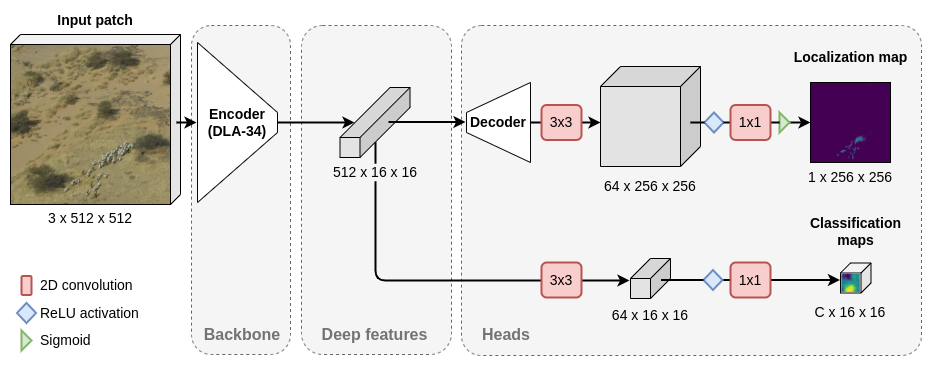
\includegraphics[width=\columnwidth]{static/img/herdnet_architecture.png} % Asegúrate de nombrar así tu archivo
%     \caption{Arquitectura de HerdNet. El modelo utiliza un backbone DLA-34 y se divide en dos cabezales: uno para generar un mapa de localización de alta resolución (arriba) y otro para mapas de clasificación de baja resolución (abajo) \cite{herdnet}.}
    \caption{HerdNet architecture. The model uses a DLA-34 backbone and is divided into two heads: one to generate a high-resolution localization map (top) and another for low-resolution classification maps (bottom) \cite{herdnet}.}
    \label{fig:herdnet_arch}
\end{figure}


% \subsubsection{Modelo Propuesto: RF-DETR}
\subsubsection{Proposed Model: RF-DETR}

% La solución propuesta se basa en \textbf{RF-DETR}, una arquitectura diseñada para optimizar el equilibrio entre precisión y latencia en aplicaciones de tiempo real. Como se ilustra en la Figura \ref{fig:rfdetr_arch}, su diseño integra componentes avanzados para mejorar la generalización y el manejo de oclusiones:
The proposed solution is based on \textbf{RF-DETR}, an architecture designed to optimize the balance between accuracy and latency in real-time applications. As illustrated in Figure \ref{fig:rfdetr_arch}, its design integrates advanced components to improve generalization and occlusion handling:

\begin{itemize}
%     \item \textbf{Backbone DINOv2:} Utiliza un \textit{Vision Transformer} (ViT-L/14) pre-entrenado con aprendizaje autosupervisado. Este backbone provee representaciones visuales robustas que facilitan la adaptación a dominios específicos con pocos datos anotados.
    \item \textbf{DINOv2 Backbone:} Uses a \textit{Vision Transformer} (ViT-L/14) pre-trained with self-supervised learning. This backbone provides robust visual representations that facilitate adaptation to specific domains with few annotated data.
%     \item \textbf{Extracción de Características Uniescala:} A diferencia de otros Transformers que procesan múltiples escalas, RF-DETR emplea una estrategia de extracción de características de una sola escala (ej. $640 \times 1280$ px) para reducir la sobrecarga computacional sin sacrificar significativamente la precisión.
    \item \textbf{Single-Scale Feature Extraction:} Unlike other Transformers that process multiple scales, RF-DETR employs a single-scale feature extraction strategy (e.g., $640 \times 1280$ px) to reduce computational overhead without significantly sacrificing accuracy.
%     \item \textbf{Cabezal Transformer y Atención Deformable:} Incorpora un mecanismo de atención cruzada deformable (\textit{Deformable Cross-Attention}) en el decodificador. Esto permite al modelo enfocarse selectivamente en características espacialmente relevantes, mejorando la detección en condiciones de oclusión severa, desorden visual (\textit{clutter}) y camuflaje, típicas de las manadas densas en la sabana.
    \item \textbf{Transformer Head and Deformable Attention:} Incorporates a \textit{Deformable Cross-Attention} mechanism in the decoder. This allows the model to selectively focus on spatially relevant features, improving detection in conditions of severe occlusion, visual \textit{clutter}, and camouflage, typical of dense herds in the savanna.
%     \item \textbf{Predicción de Conjuntos sin NMS:} El modelo realiza una predicción directa de conjuntos de cajas delimitadoras, eliminando la necesidad de anclajes (\textit{anchor boxes}) y de la Supresión de No Máximos (NMS). Esto es crítico para resolver el problema de subconteo en manadas densas, donde el NMS tradicional suprimiría detecciones válidas muy próximas.
    \item \textbf{Set Prediction without NMS:} The model performs direct set prediction of bounding boxes, eliminating the need for \textit{anchor boxes} and Non-Maximum Suppression (NMS). This is critical to solve the undercounting problem in dense herds, where traditional NMS would suppress valid detections in close proximity.
%     \item \textbf{Variantes:} Para evaluar el compromiso entre precisión y costo, se implementaron tres variantes: Nano (384 px), Small (512 px) y Large (560 px), permitiendo adaptar la complejidad del modelo a los recursos disponibles.
    \item \textbf{Variants:} To evaluate the tradeoff between accuracy and cost, three variants were implemented: Nano (384 px), Small (512 px), and Large (560 px), allowing the model complexity to be adapted to available resources.
\end{itemize}

\begin{figure*}[ht]
    \centering
    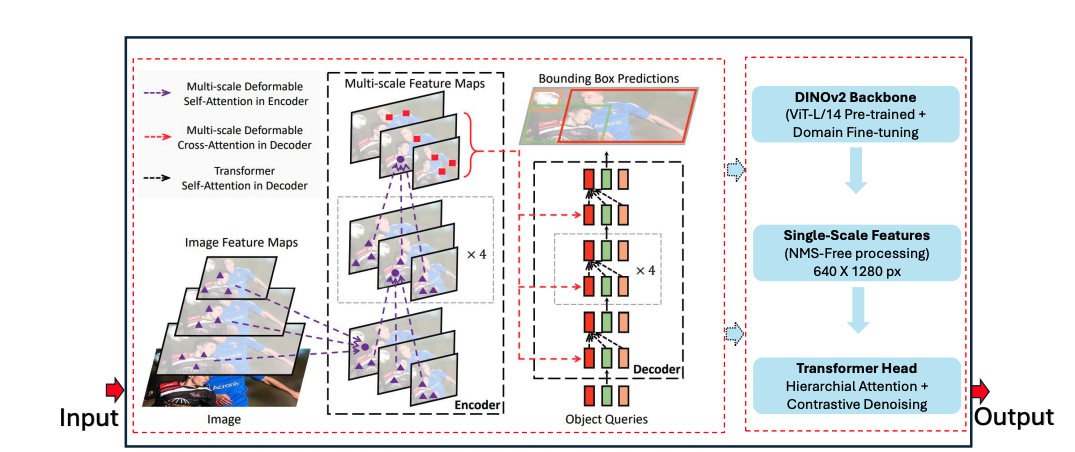
\includegraphics[width=0.93\textwidth]{static/img/rfdetr_architecture.png}
%     \caption{Arquitectura de RF-DETR para la detección de objetos. Muestra el flujo desde el backbone DINOv2, pasando por la extracción de características uniescala, hasta el cabezal Transformer con atención jerárquica y eliminación de ruido contrastivo. \cite{rf-detr}}
    \caption{RF-DETR architecture for object detection. Shows the flow from the DINOv2 backbone, through single-scale feature extraction, to the Transformer head with hierarchical attention and contrastive noise elimination. \cite{rf-detr}}
    \label{fig:rfdetr_arch}
\end{figure*}


% \subsection{Estrategia de Entrenamiento}
\subsection{Training Strategy}

\begin{figure}[ht]
    \centering
    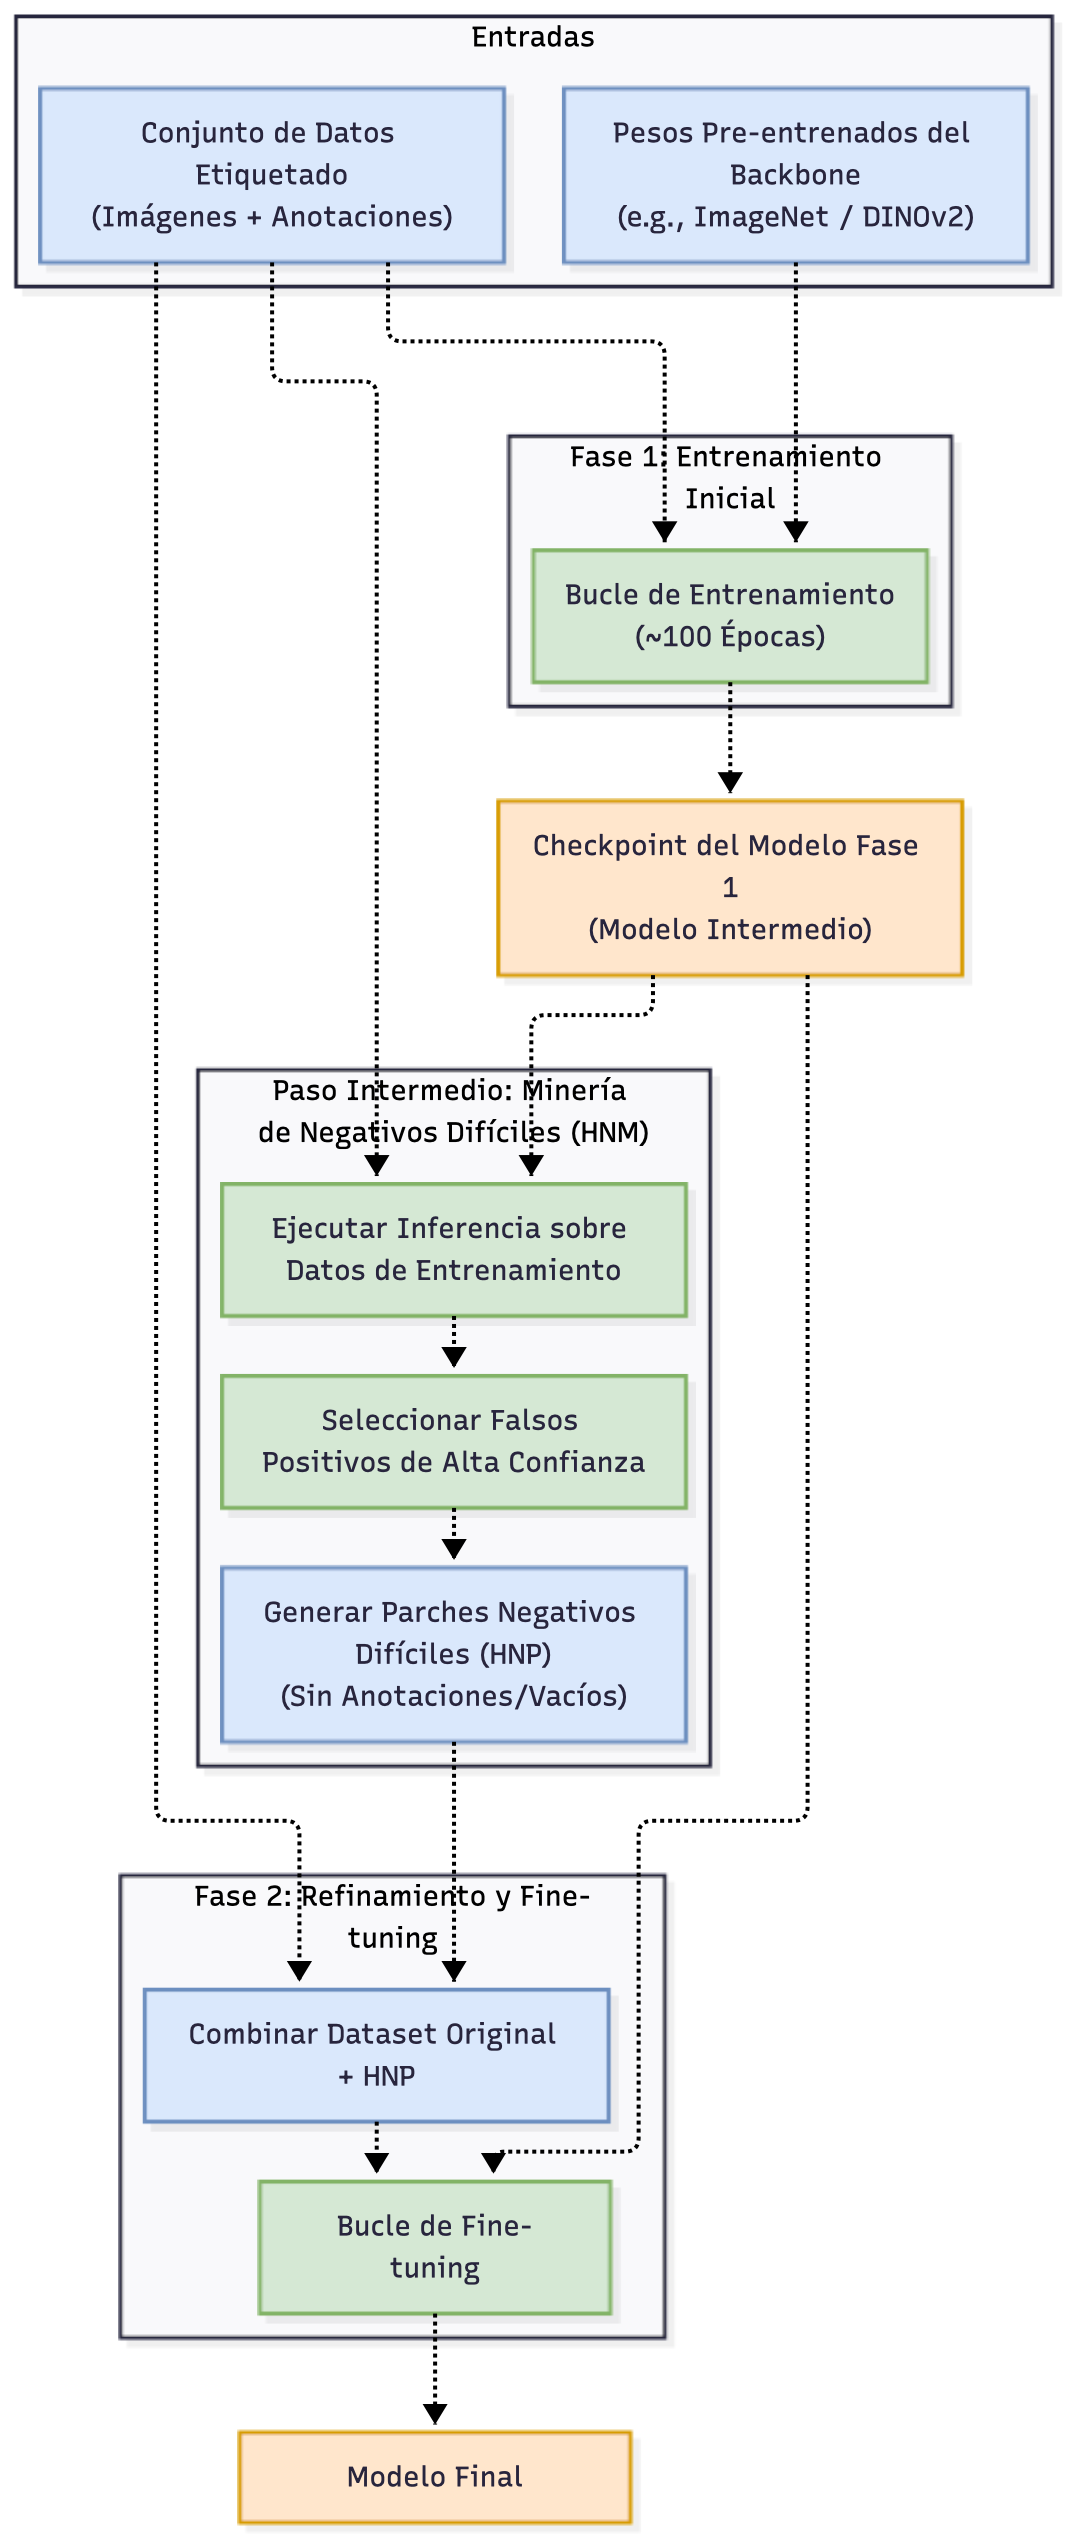
\includegraphics[width=0.35\textwidth, height=0.48\textheight]{static/img/entrenamiento.png}
%     \caption{Flujo de entrenamiento.}
    \caption{Training flow.}
    \label{fig:deployment_arch}
\end{figure}


% Se diseñó un protocolo dividido en dos etapas principales: la replicación del \textit{baseline} y el entrenamiento especializado del modelo propuesto, adaptando la técnica de minería de negativos difíciles (\textit{Hard Negative Mining}) para maximizar la precisión.
A protocol was designed divided into two main stages: the replication of the \textit{baseline} and the specialized training of the proposed model, adapting the \textit{Hard Negative Mining} technique to maximize accuracy.

% \subsubsection{Replicación de HerdNet}
\subsubsection{HerdNet Replication}

% El proceso se realizó en dos fases secuenciales:
The process was carried out in two sequential phases:
\begin{enumerate}
%     \item \textbf{Fase 1 (Entrenamiento Inicial):} Se entrenó el modelo durante 100 épocas con un \textit{learning rate} inicial de $1\times10^{-4}$ y un optimizador AdamW. La función de pérdida combinó \textit{Focal Loss} para la localización y \textit{Cross Entropy Loss} ponderada para la clasificación, asignando pesos específicos ($w=[0.1; 1.0; 2.0; \dots]$) para mitigar el desbalance de clases.
    \item \textbf{Phase 1 (Initial Training):} The model was trained for 100 epochs with an initial \textit{learning rate} of $1\times10^{-4}$ and an AdamW optimizer. The loss function combined \textit{Focal Loss} for localization and weighted \textit{Cross Entropy Loss} for classification, assigning specific weights ($w=[0.1; 1.0; 2.0; \dots]$) to mitigate class imbalance.
%     \item \textbf{Fase 2 (Refinamiento con HNP):} Se realizó un segundo entrenamiento de 50 épocas con una tasa de aprendizaje reducida a $1\times10^{-6}$. En esta etapa se introdujeron los parches negativos difíciles (\textit{Hard Negative Patches} - HNP), generados al ejecutar el modelo de la Fase 1 sobre las imágenes de entrenamiento y recolectar las predicciones de falsos positivos con alta confianza.
    \item \textbf{Phase 2 (Refinement with HNP):} A second training of 50 epochs was performed with a learning rate reduced to $1\times10^{-6}$. In this stage, \textit{Hard Negative Patches} (HNP) were introduced, generated by running the Phase 1 model on the training images and collecting high-confidence false positive predictions.
\end{enumerate}

% \subsubsection{Adaptación para RF-DETR}
\subsubsection{Adaptation for RF-DETR}

% Se replicó la estrategia de dos fases de HerdNet con las siguientes adaptaciones para la arquitectura Transformer:
The two-phase strategy of HerdNet was replicated with the following adaptations for the Transformer architecture:

% \paragraph{Hiperparámetros de Entrenamiento}
\paragraph{Training Hyperparameters}

% \textbf{Fase 1:} Se utilizó el \textit{backbone} DINOv2 pre-entrenado con normalización ImageNet y learning rate por defecto del framework (con decaimiento por capas). Se implementó un callback personalizado para monitorear métricas de HerdNet durante el entrenamiento.
\textbf{Phase 1:} The pre-trained DINOv2 \textit{backbone} was used with ImageNet normalization and the framework's default learning rate (with layer-wise decay). A custom callback was implemented to monitor HerdNet metrics during training.

% \textbf{Fase 2:} Fine-tuning con learning rate reducido ($1 \times 10^{-5}$ para las tres variantes), aumentación multi-escala activada, y regularización mediante weight decay y EMA. El dataset ampliado con HNP mantuvo las anotaciones originales solo en los parches positivos, forzando al modelo a predecir ausencia de objetos en regiones visualmente confusas.
\textbf{Phase 2:} Fine-tuning with reduced learning rate ($1 \times 10^{-5}$ for the three variants), multi-scale augmentation enabled, and regularization through weight decay and EMA. The dataset augmented with HNP maintained the original annotations only in positive patches, forcing the model to predict absence of objects in visually confusing regions.


% \paragraph{Inferencia y Evaluación}
\paragraph{Inference and Evaluation}

% Se empleó un \texttt{SimpleStitcher} para procesar imágenes completas en ventanas deslizantes y reconstruir detecciones en coordenadas originales. Las métricas se calcularon con el framework de HerdNet (radio de 20 píxeles) para mantener comparabilidad directa.
A \texttt{SimpleStitcher} was used to process complete images in sliding windows and reconstruct detections in original coordinates. Metrics were calculated with the HerdNet framework (20-pixel radius) to maintain direct comparability.

% \subsection{Herramientas y Despliegue}
\subsection{Tools and Deployment}

% El desarrollo de la solución siguió una arquitectura de microservicios modular, separando el motor de inferencia de la capa de presentación y orquestando el despliegue mediante prácticas de Infraestructura como Código (IaC).
The solution development followed a modular microservices architecture, separating the inference engine from the presentation layer and orchestrating the deployment through Infrastructure as Code (IaC) practices.

% \subsubsection{Backend y Optimización de Inferencia}
\subsubsection{Backend and Inference Optimization}

% El núcleo del sistema se implementó utilizando \textbf{FastAPI}, exponiendo una API REST de alto rendimiento. Para optimizar la latencia en un entorno de producción, se migró el modelo entrenado en PyTorch al formato \textbf{ONNX Runtime}. Esta decisión técnica permitió:
The system core was implemented using \textbf{FastAPI}, exposing a high-performance REST API. To optimize latency in a production environment, the model trained in PyTorch was migrated to the \textbf{ONNX Runtime} format. This technical decision allowed:
\begin{itemize}
%     \item Maximizar la velocidad de inferencia, reduciendo la dependencia de GPUs costosas en inferencia.
    \item Maximize inference speed, reducing dependence on expensive GPUs for inference.
%     \item Disminuir la huella de memoria y garantizar la portabilidad entre diferentes arquitecturas de hardware.
    \item Reduce memory footprint and ensure portability across different hardware architectures.
\end{itemize}
% La API gestiona endpoints críticos como \texttt{/api/inference} para el procesamiento de imágenes y \texttt{/health} para el monitoreo de disponibilidad.
The API manages critical endpoints such as \texttt{/api/inference} for image processing and \texttt{/health} for availability monitoring.

% \subsubsection{Interfaz de Usuario (Frontend)}
\subsubsection{User Interface (Frontend)}

% Para la validación visual y comparación de experimentos, se desarrolló una \textit{Single Page Application} (SPA) basada en el stack moderno de \textbf{React} y \textbf{TypeScript}, construida con Vite. La interfaz integra:
For visual validation and experiment comparison, a \textit{Single Page Application} (SPA) was developed based on the modern stack of \textbf{React} and \textbf{TypeScript}, built with Vite. The interface integrates:
\begin{itemize}
%     \item \textbf{Visualización de Detecciones:} Componentes de Canvas personalizados para renderizar las cajas delimitadoras (\textit{bounding boxes}) sobre las imágenes aéreas de alta resolución.
    \item \textbf{Detection Visualization:} Custom Canvas components to render \textit{bounding boxes} on high-resolution aerial images.
%     \item \textbf{Comparativa de Modelos:} Módulos específicos (\textit{ExperimentComparison}) que permiten contrastar visualmente el rendimiento entre diferentes versiones del modelo (e.g., RF-DETR vs. Baseline).
    \item \textbf{Model Comparison:} Specific modules (\textit{ExperimentComparison}) that allow visual contrast of performance between different model versions (e.g., RF-DETR vs. Baseline).
\end{itemize}

% \subsubsection{Infraestructura Cloud y Orquestación}
\subsubsection{Cloud Infrastructure and Orchestration}

% El despliegue en producción se realizó sobre \textbf{Amazon Web Services (AWS)}, utilizando \textbf{Terraform} para garantizar la reproducibilidad de la infraestructura. La arquitectura, diseñada para alta disponibilidad y eficiencia de costos, se compone de:
The production deployment was performed on \textbf{Amazon Web Services (AWS)}, using \textbf{Terraform} to ensure infrastructure reproducibility. The architecture, designed for high availability and cost efficiency, consists of:

\begin{enumerate}
%     \item \textbf{Cómputo Serverless (AWS ECS \& Fargate):} La aplicación se contenedorizó con Docker y se desplegó en Amazon ECS utilizando la estrategia de capacidad \textit{Fargate Spot}, logrando una reducción de costos operativa estimada del 70\%.
    \item \textbf{Serverless Computing (AWS ECS \& Fargate):} The application was containerized with Docker and deployed on Amazon ECS using the \textit{Fargate Spot} capacity strategy, achieving an estimated operational cost reduction of 70\%.
%     \item \textbf{Gestión de Tráfico:} Se implementó un \textit{Application Load Balancer} (ALB) distribuido en múltiples zonas de disponibilidad, con verificaciones de estado automáticas para gestionar el tráfico de inferencia.
    \item \textbf{Traffic Management:} An \textit{Application Load Balancer} (ALB) distributed across multiple availability zones was implemented, with automatic health checks to manage inference traffic.
%     \item \textbf{Seguridad y Monitoreo:} La red se aisló mediante una VPC privada, restringiendo el acceso a los contenedores únicamente a través del ALB. El monitoreo de logs y métricas de rendimiento se centralizó en \textit{CloudWatch}, asegurando la observabilidad del sistema en tiempo real.
    \item \textbf{Security and Monitoring:} The network was isolated through a private VPC, restricting access to containers only through the ALB. Log monitoring and performance metrics were centralized in \textit{CloudWatch}, ensuring real-time system observability.
\end{enumerate}

\begin{figure}[ht]
    \centering
    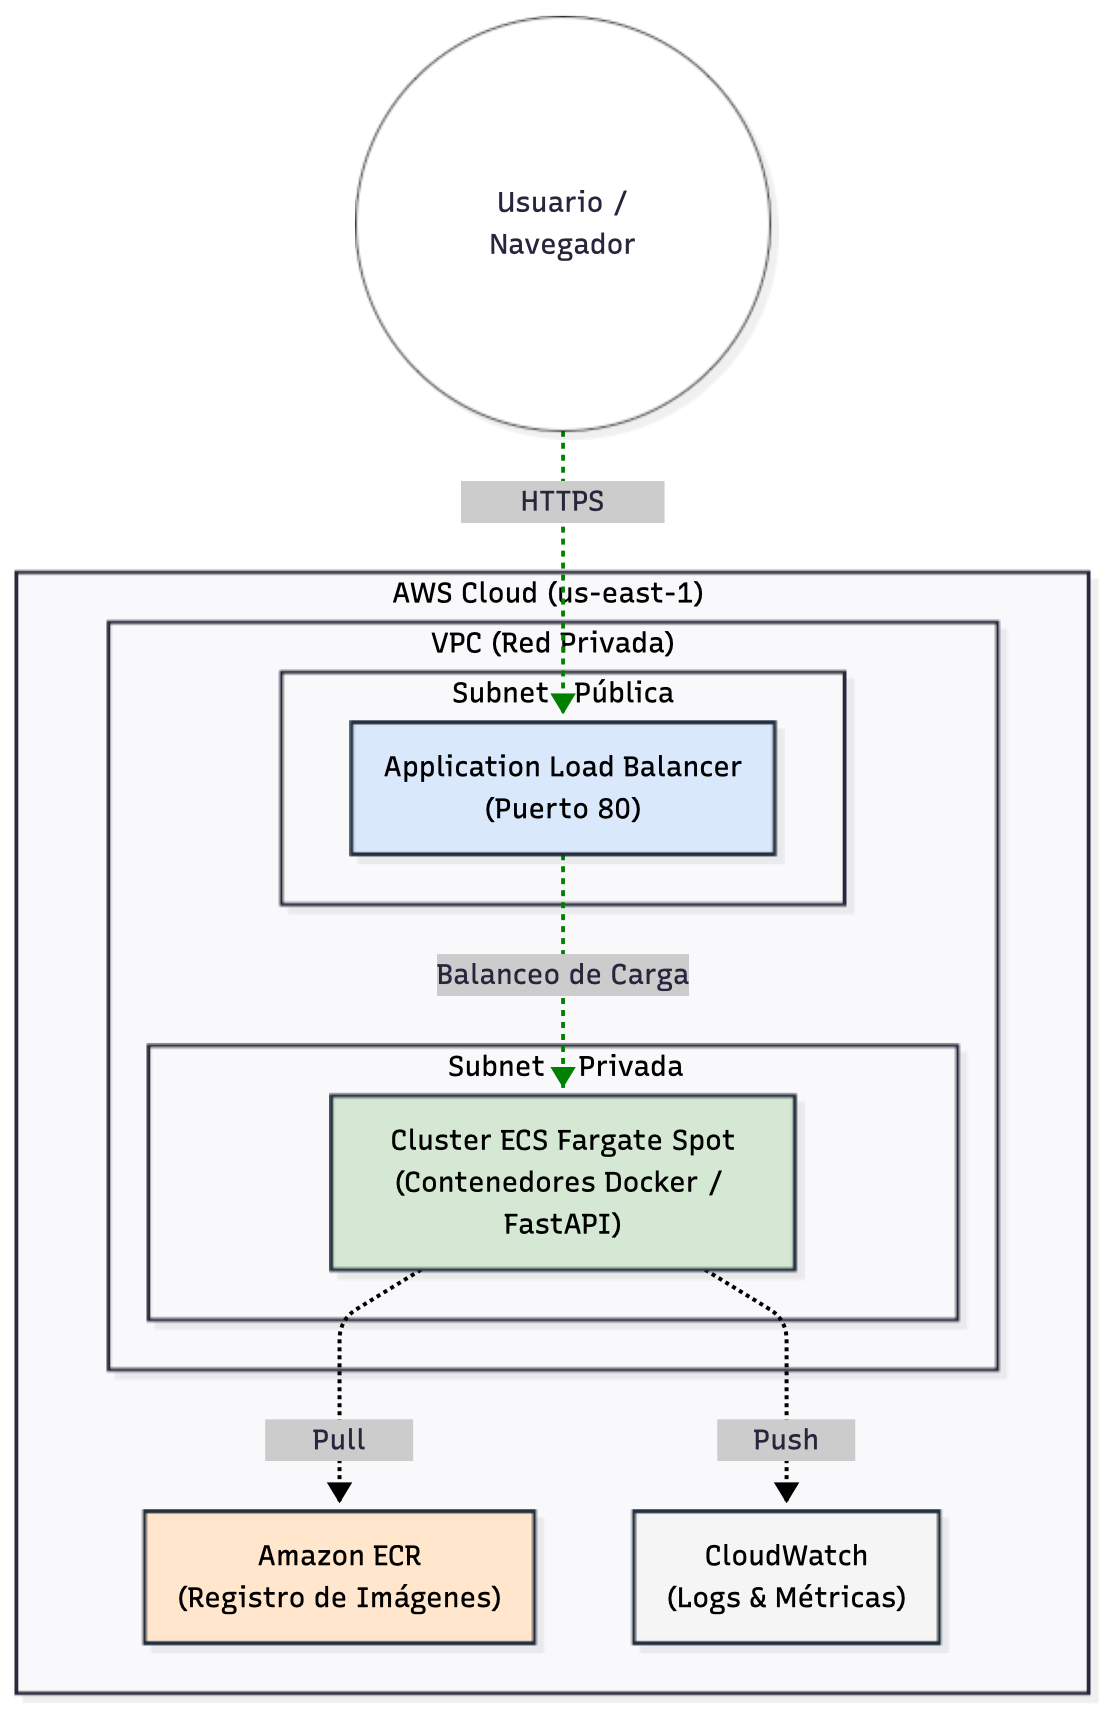
\includegraphics[width=0.4\textwidth]{static/img/arquitectura_despliegue.png}
%     \caption{Arquitectura de despliegue de la solución en la nube.}
    \caption{Cloud deployment architecture of the solution.}
    \label{fig:deployment_arch}
\end{figure}
